%
% include the class file for USI-INF Technical Reports
%
\documentclass{usiinftr}
\usepackage{float}
\usepackage{amsmath}
\usepackage{slashbox}
\usepackage{subfigure}

%
% if you want to create a cover page only (e.g. to put it in front
% of a WORD document or the like), use the "coverpage" option
%
%\documentclass[coverpage]{usiinftr}

%%%%%%%%%%%%%%%%%%%%%%%%%%%%%%%%%%%%%%%%%%%%%%%%%%%%%%%%%%%%%%%%%%%%

\begin{document}

\title{\bf Particle Simulations with OpenACC: Speedup and Scaling}

%\author{Lawrence Farinola}{1}
\author{Samuel A. Cruz Alegría, Alessandra M. de Felice, Hrishikesh R. Gupta}{1}

\affiliation{1}{\USIINF}

%
% put the number of your Technical Report here; in order to determine
% the number, take the number of the most recent USI INF Technical Report
% (on top of the list at http://www.inf.usi.ch/techreports/) and increment
% it by one; the format is "[year]-[number]"
%
\TRnumber{2013-3}

%
% by default, the current month and year are used as the publication date
% of your Technical Report; if you want to change this, then you can do it here, e.g.
%
%\date{February~\the\year}
%\date{August 2011}

\maketitle

\begin{abstract}
The simulation of particle systems has become essential for visualizing the behaviour of relevant physical systems, ranging from simulations of molecular dynamics to simulations of colliding galaxies. The computational complexity of performing simulations grows with the number of particles in the system. Performing realistic simulations may necessitate a plethora of particles, leading to immense computational costs. Simulating such systems may thus require increasingly longer time frames. Hence, performing increasingly complex sim- ulations may become impractical for single-core simulation tools. Thus, it is essential to develop simulation tools which perform practically independent of the number of bodies used in a simulation. A possibility to reduce the time required for simulations is to distribute the workload among different parallel entities, such as different processes or threads. This paper aims to explore the efficiency and scalability of parallelization in order to improve the performance of a simulation currently run on a single core. This is achieved by incorpo- rating the OpenACC programming standard, which is a programming standard for parallel computing that utilizes a hardware accelerator, such as a GPU.
\end{abstract}

\section{Introduction}
Tsunamis belong to the most devastating ocean disasters in the world. When they reach the dense-populated  
coastline areas unexpectedly, fatal destructions and lot of deads are claimed. In order to prevent
such scenarios, it is required to have a tool that would provide fast and detailed simulation of tsunami.
One of the models that could be used for tsunami simulation is SWE model \cite{swe, BreuerB12}. 

Tsunamis are massive oceanic waves generated by underwater earthquakes. The earthquakes are caused by
collision of multiple tectonic plates. During such events plates are usually slipped over each other or deformed
in that way they cause the displacement of the sea floor and increase of the water level. The resulting
tsunami propagates into all directions from the source region by gravitational force. This study deals
with Sumatra 2004 and T\={o}hoku 2011 tsunamis.

Shallow water equations \cite{nummethods} (the underlying mathematical concept of the {SWE} model) describe the behavior of a fluid, in particular water, in a two-dimensional domain.
The main modeling  assumption of the equations is that we can neglect effects of flow in vertical direction. This conditions 
holds if we think of ocean in global terms, i.e., horizontal lengths  are much greater than vertical lengths (the ocean depth).
Shallow water equations describe the change of water depth $h$ and horizontal velocities $v_x$ and $v_y$  over time,  depending on some
initial conditions, in this case -- ocean floor displacement during the earthquake. The respective changes
of water depth $h$ in time can be described by a system of partial differential~equations \eqref{eq:swe}.

High-resolution tsunami simulations result into large problems, that could often be solved in reasonable time only using parallel
computations. This study is aimed to find the most efficient configuration and evaluate performance
of emerging massively-parallel graphics processing units (GPUs).

The paper is organized as follows. Section \ref{sec:methodology} provides description of used data and earthquake model.
It describes their meaning, origin, transformations and how the data were used in order to obtain the result.
Section \ref{sec:experiments} provides experimental results and analyses the credibility of performed simulations.
Speedup and parallel efficiency of different SWE configurations are discussed in Section \ref{sec:benchmarking}.

\begin{equation} \left\{
  \begin{array}{l} \label{eq:swe}
     \displaystyle \frac{\partial h}{\partial t} + \frac{\partial (v_x h)}{\partial x} + \frac{\partial (v_y h)}{\partial y} \enskip = \enskip 0,  \\[1em]
     \displaystyle \frac{\partial (h v_x)}{\partial t} + \frac{\partial (h v_x v_x)}{\partial x}  + \frac{\partial (h v_y v_x)}{\partial y}
         + \frac{1}{2} g \frac{\partial (h^2)}{\partial x}  \enskip = \enskip - gh \frac{\partial b}{\partial x}, \\[1em]
      \displaystyle \frac{\partial (h v_y)}{\partial t} + \frac{\partial (h v_x v_y)}{\partial x}  + \frac{\partial (h v_y v_y)}{\partial y}
         + \frac{1}{2} g  \frac{\partial (h^2)}{\partial y} \enskip = \enskip - gh \frac{\partial b}{\partial y}, \\[1em]
      \displaystyle h|_{t=0}(x,y) = h_0(x,y).
  \end{array}
  \right.
\end{equation}

\section{Simulation methodology}
\label{sec:methodology}

The basic flow of the simulation pipeline is shown in the Figure \ref{fig:flowchart}. The skewed rectangles represent data files and the
regular rectangles with double vertical borders represent applications and tools. 

\begin{figure}[H]
\begin{center}
  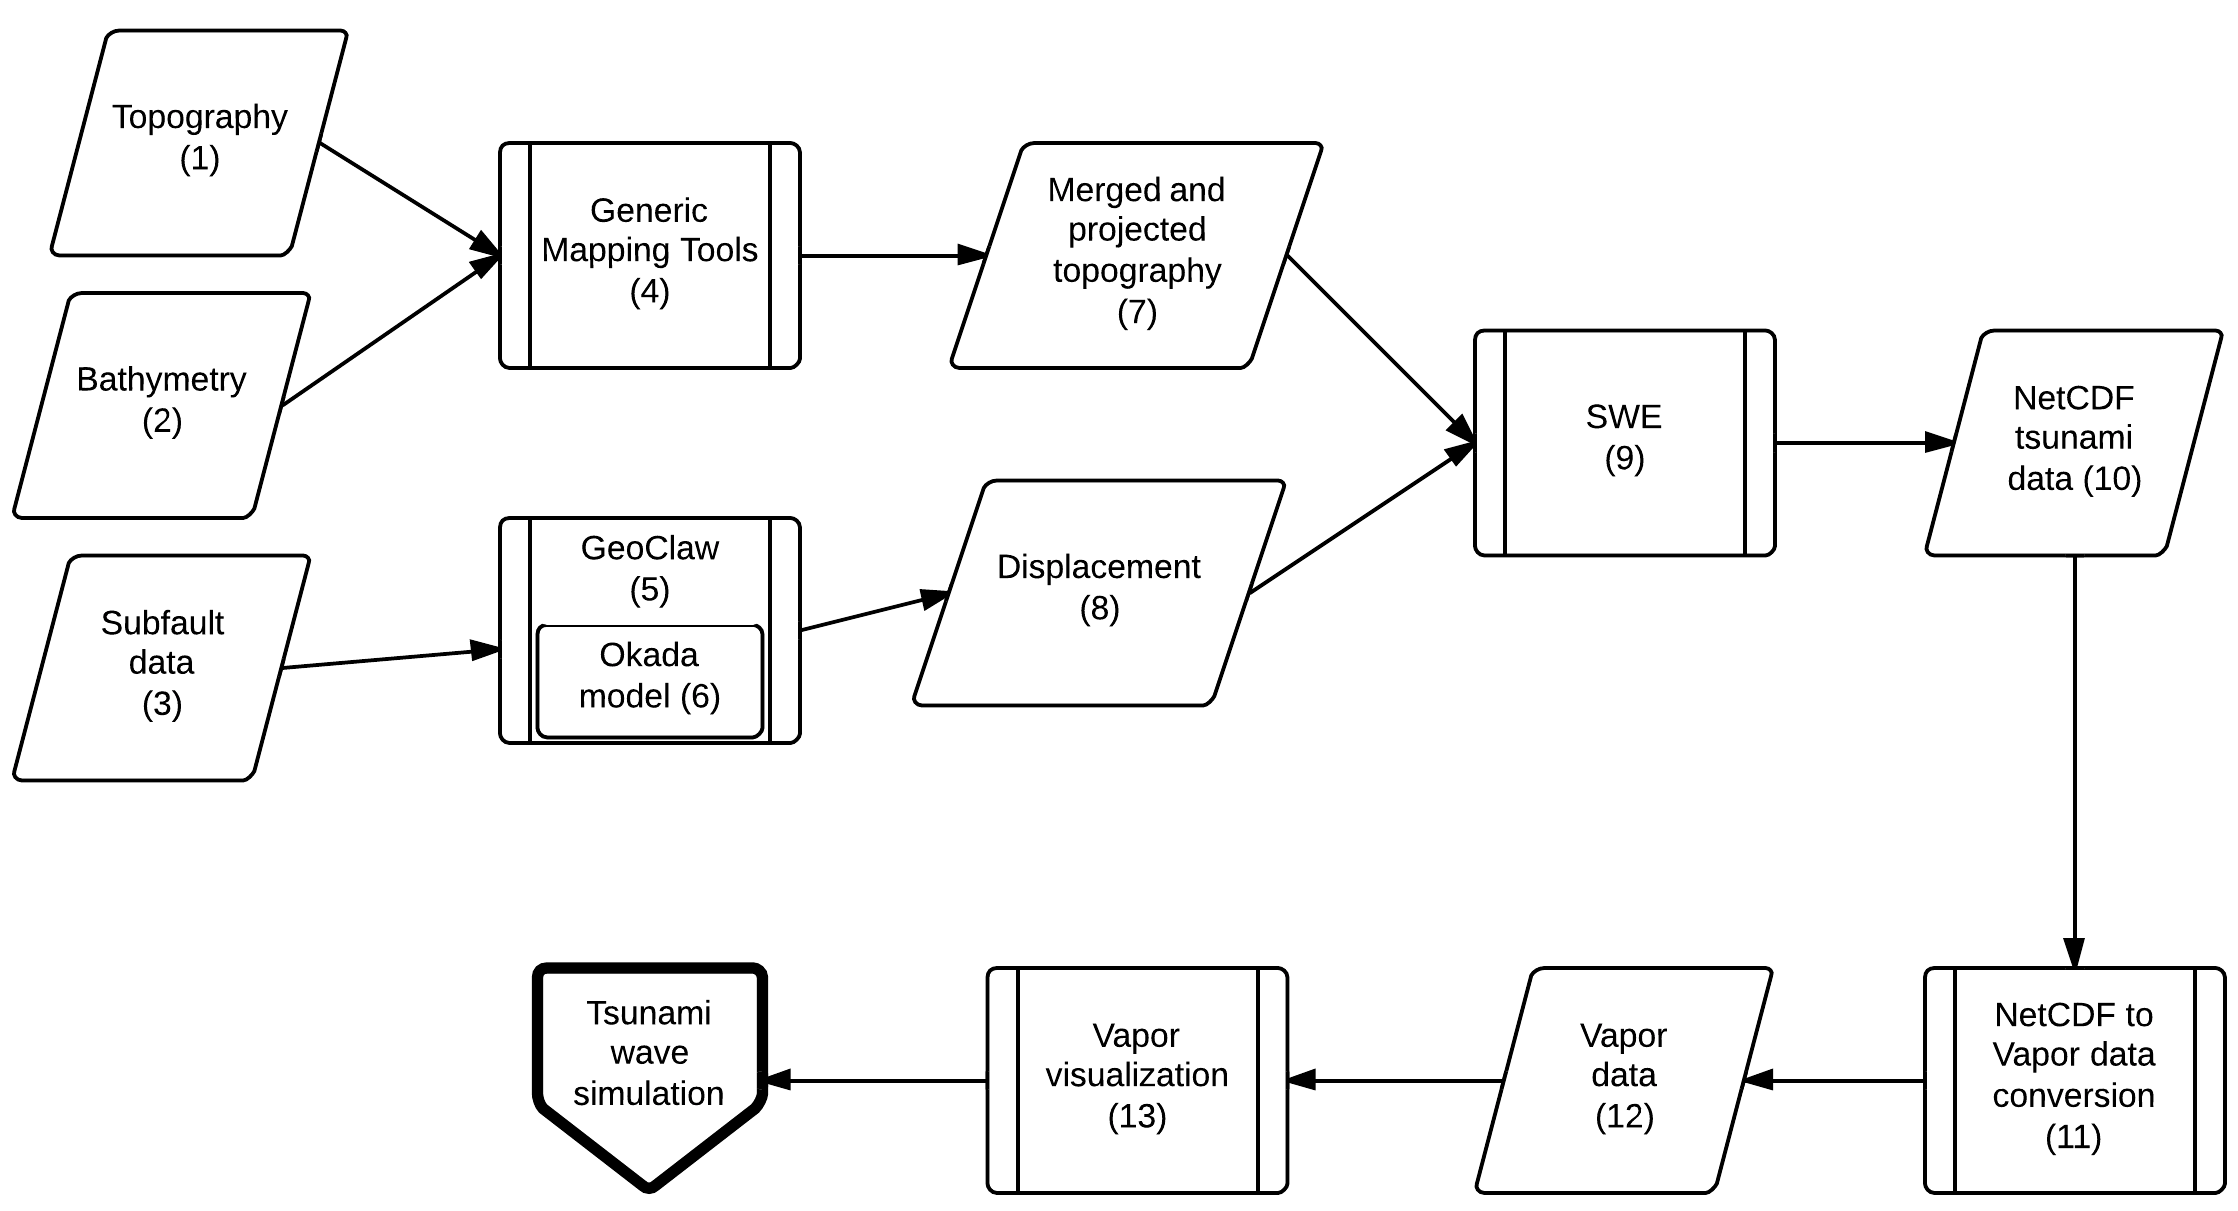
\includegraphics[width=1\textwidth]{figures/PDCPipeline}
  \caption{Simulation methodology flowchart of components \label{fig:flowchart}}  
\end{center}
\end{figure}

\subsection{Input files and preprocessing}

In the SWE model tsunami is identified by the number of input data fields. First of all,
we need the model of the Earth's surface including the mainland as well as the ocean floor (items (1) and (2) in Figure \ref{fig:flowchart}).
ETOPO1 \cite{etopo1} Global Relief Model is a 1 arc-minute (\textasciitilde 1.8 km) model of Earth's surface that integrates land topography and ocean bathymetry.
The global 30 arc-second grid (\textasciitilde 0.9 km) ocean floor relief (bathymetry) is provided by GEBCO \cite{GEBCO}.

The relief data cannot be used by the SWE in the raw form. The basic data structure of the SWE is a rectangular plain grid. The bathymetry (2)
and topography (1) data need to be projected on the grid (7) including the whole region of interest. For this purpose Generic Mapping Tools (4)
are used. GMT merge topography and bathymetry data and generate the rectangular grid of region (7) defined by latitude and longitude coordinates.

We also need a model of the seismic event that triggered the tsunami. The tsunami is initiated when the sea floor displacement  occurs.
We need to know several aspects of the event including the exact area of the sea floor that was displaced, how much it was displaced
and the time and direction of the movement. The movement of the sea floor is estimated using various sensor measurements
in the area affected by the earthquake. These measurements are usually maintained by U.S. Geological Survey, which also provides
the data in several formats. The SWE is configured for the subfault format (3). 

In case of the tsunami simulation we are not interested in the seismic activity itself. We only need to know the initial displacement
of the sea floor, i.e. the initial state of the tsunami wave. The resulting wave propagation can be computed with SWE model. To get the displacement (8) we need to transform the subfault data (3). This transformation
is defined in the Okada model (6) \cite{okada}, which is analytical model for computing displacement from subfault and is a part of GeoClaw pack (5) \cite{geoclaw}.
It predicts surface displacement according to a specified rectangular dislocation at depth using Green's functions.
According to \cite{okada1}, Okada model may be sufficient for simulating large intra-continental earthquakes but
it has limitations in simulating small area earthquakes.

\subsection{Postprocessing and visualization}
The result of simulation is encoded in NetCDF format (10). The NetCDF encodes data in the self-describing
and machine independent manner. When SWE used in parallel mode a separate NetCDF file is created for each MPI process.
We visualize the simulation output with {VAPOR}, which eases the process by compressing the huge amount of original NetCDF data,
yet conserving most of the important detail. The conversion step (11) could be done on server resulting into much smaller
file to be transferred and visualized on user machine (12-13).

\section{Experimental results}
\label{sec:experiments}

\begin{figure}
\centering
\mbox{
\subfigure[Propagation of Sumatra 2004 tsunami wave]{
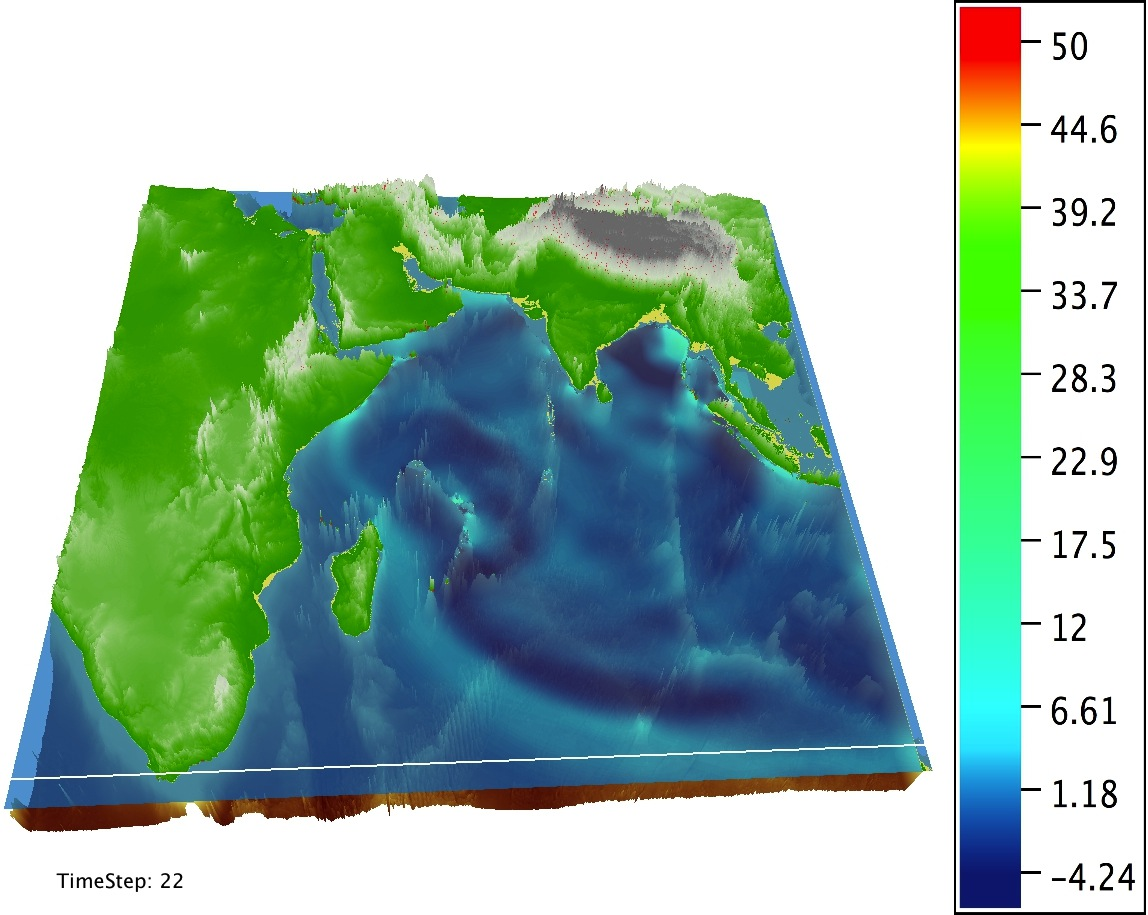
\includegraphics[height=6cm]{figures/aaa.jpg} 
\label{fig:sumatra}
}}
\quad
\mbox{
\subfigure[Propagation of T\={o}hoku 2011 tsunami wave]{
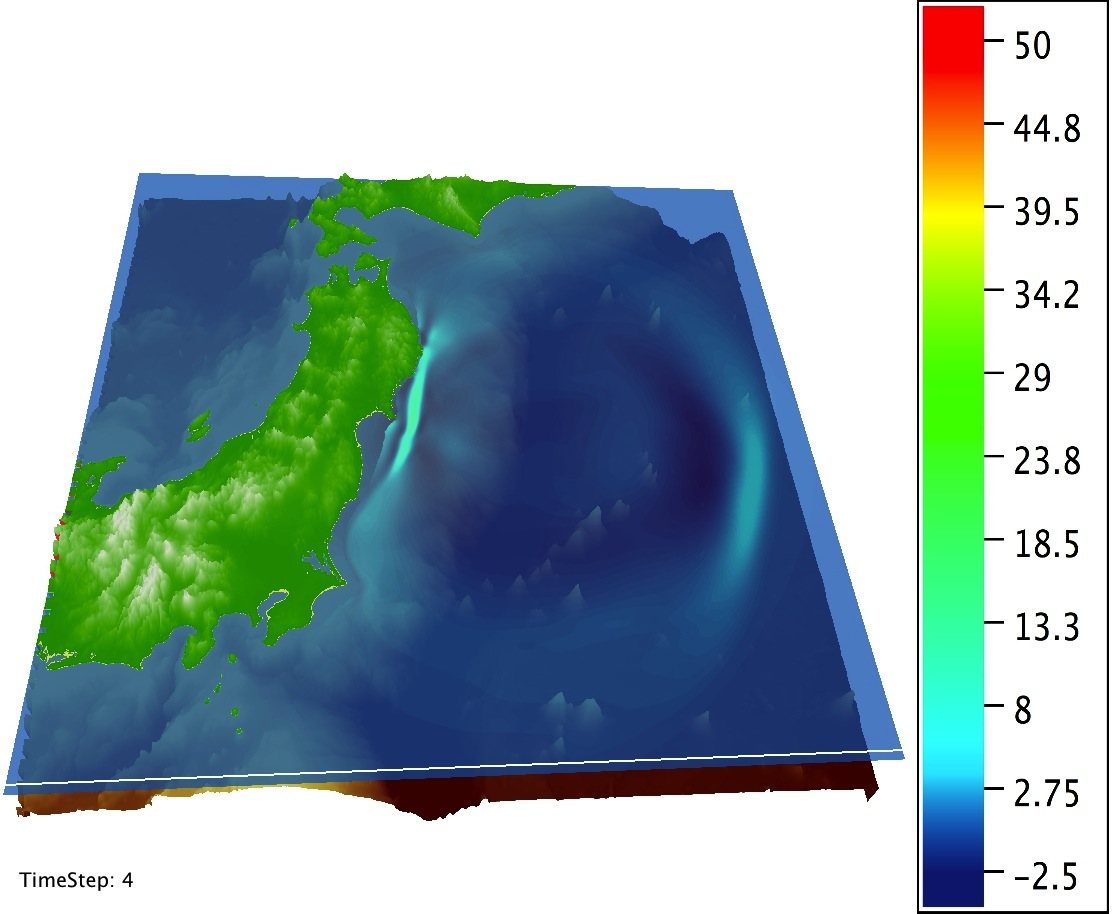
\includegraphics[height=6cm]{figures/bbb.jpg}
\label{fig:tohoku}
}}
\caption{Visualization of tsunami waves}
\label{fig:visualization}
\end{figure}

The Great Sumatra--Andaman earthquake of December 26th, 2004 occurred on the interface of the India and Burma plates
and was caused by the release of stresses that develop as the India plate subducts beneath the overriding
Burma plate. An estimated 1,600 kilometers  of fault surface slipped about 15 meters
along the subduction zone where the Indian Plate slides under the overriding Burma Plate. The sudden vertical
rise of the seabed during the earthquake displaced massive volumes of water, resulting in a tsunami
that struck the coasts of the Indian Ocean. The tsunami was noticed as far as Struisbaai in South Africa,
8,500 km away, where a 1.5 m high tide surged on shore about 16 hours after the earthquake \cite{sumatra}.

In case of great Sumatra--Andaman earthquake and tsunami the rupture process was estimated using tsunami waveforms observed at
tide gauges and the coseismic vertical deformation observed along the coast \cite{sumatraPaper}. The tsunami waveform inversion was used to estimate the slip
distribution of the earthquake. The fault area of the earthquake is divided into several smaller subfaults and the slip amount on each subfault
is estimated from the observed tsunami waveforms. 

The magnitude 9.0 Tohoku earthquake on March 11, 2011, which occurred near the northeast coast of Honshu, Japan,
resulted from thrust faulting on or near the subduction zone plate boundary between the Pacific and North America plates.
Modeling of the rupture of this earthquake indicate that the fault moved upwards of 30-40 m, and slipped over an area
approximately 300 km long (along-strike) by 150 km wide (in the down-dip direction) \cite{tohoku}.
The tsunami propagated throughout the Pacific Ocean region reaching the entire Pacific coast of North and South America
from Alaska to Chile. Tsunami around the coastline of Japan reached heights from 3 to 6 m.

Simulation of the tsunami wave propagation can begin after the initial sea floor displacement (7) and initial waveform have been computed.
Propagation model and the behavior  of the wave is defined in the SWE model.
Wave propagation is simulated for specified time range and on specific area of interest defined relative to the epicenter. SWE is able
to adapt time step for numerical stability conditions. Visualization of wave propagation can be seen in Figure \ref{fig:visualization}.

SWE can be configured to run in parallel or to use GPU accelerators in order to speed up the simulation. Detailed description of used configurations and the resulting speed up and efficiency is discussed in the section \ref{sec:benchmarking}.  



\subsection{Credibility of performed tsunami simulations}
Credibility of the performed tsunami simulations has been verified by comparison to numerous reports containing the
list of mainland areas hit by tsunami, observations of the tsunami wave and ocean level sensors measurements.

The great Sumatra--Andaman tsunami has been observed in 14 countries in South Asia and East Africa.
The tsunami caused more casualties than any other in recorded history and was recorded nearly world-wide
on tide gauges in the Indian, Pacific and Atlantic Oceans. Seiches were observed in India and the United States.
Subsidence and landslides were observed in Sumatra \cite{sumatra}. According to our SWE results, the tsunami wave reveals the propagation
through the whole Indian Ocean and shows the wave hitting the adjacent coastline areas. Wave continues to propagate
through the open ocean reaching the coastline of Africa. On its arrival on shore, the height of the tsunami varied greatly,
depending on its distance and direction from the epicentre and other factors such as the local bathymetry.
Reports have the height ranging form 2-3 m at the African coast near Kenya \cite{africa_tsunami}.
Simulation revealed the height of tsunami waves reaching the Kenyan coastline of approximately the same height.
The tsunami was observed also in Struisbaai, South Africa, where a 1.5 m high tide surged on shore \cite{sumatra}.
Similar results were observed in the simulation.

In the case of T\={o}hoku, the majority of casualties and damage occured in Iwate, Miyagi and Fukushima from a Pacific-wide
tsunami with a maximum runup height of 37.88 m at Miyako. The tsunami destroyed or severely damaged many coastal towns in the
Kuji-Minamisanriku-Nami area \cite{tohoku}. According to our SWE results, tsunami
was spreading in the direction of the most affected islands of Honshu and Hokkaido but the wave was eliminated just before reaching
the coastline areas. This behavior is probably caused by some numerical constraing in the SWE model.

\section{Benchmarking} 
\label{sec:benchmarking}
The SWE has been run with different configurations to find out the most efficient settings. SWE was used in 
parallel mode with 1 to 8 MPI processes and also with GPUs included. The simulations were run on two different
clusters: Tesla-CMC, equipped with {NVIDIA} Tesla C2075 GPUs and Todi Cray XK-7, equipped with
{NVIDIA} K20 GPUs. The summarization of the speedups can be found in the Table \ref{tab:tohoku_speedup}, \ref{tab:sumatra_speedup} and \ref{tab:todi_speedup};
Table \ref{tab:efficiency} presents the efficiency of different configurations.

It is obvious from results that when higher degree of parallelism  is used the speedup is increased but
the efficiency is decreasing because of the inter-process communication. When the GPU is used the
speedup increases dramatically. When multiple GPUs are used, speedup continues to increase, while
the efficiency only slightly decreases.

\section{Conclusion} 
In this paper we presented the realistic tsunami simulations with an emphasis on how fast and detailed solution could be achieved on emerging parallel architectures. Such simulations are
important for analysis and prediction of catastrophical scenarios in dense-populated areas reachable by tsunamis.

The propagation of the tsunami wave is computed using the SWE water wave propagation model.
The SWE model works with subfault earthquake model from which is computed
initial sea floor displacement using Okada transformation. Several data files with representation of
ocean bathymetry and mainland topography are needed for the simulation. Great Sumatra--Andaman tsunami of 2004 and
T\={o}hoku 2011 tsunami simulations have been performed.
 
The SWE model has been run with different configurations to benchmark the performance of the GPU-enabled clusters Tesla-CMC and Todi Cray XK-7. SWE model has been run in parallel mode with multiple CPU processes with and without using GPUs. The performance of the massively-parallel graphics processing units (GPUs) have shown impressive results. Using all available GPUs, we observed the maximum speedup of 158x in comparison to single-core CPU version. The most efficient configuration was the one with a single GPU, achieving speedup of 58x. 

\emph{I would like to thank Dmitry Mikushin of the University of Lugano, Sebastian Rettenberger and Alexander Breuer of SWE model development team for their help with the various technical issues. Imagery produced by VAPOR (www.vapor.ucar.edu), a product of the Computational Information Systems Laboratory at the National Center for Atmospheric Research. This study has been performed as a part of ``Parallel \& Distributed Computing Lab'' course in the University of Lugano.}

\bibliographystyle{plain}
\bibliography{citations}

\begin{table}
\begin{center}
\begin{tabular}{|l||r|r|r|r|r|r|r|r|} \hline
\backslashbox{\bf Config}{\bf Process} & 0 & 1 & 2 & 3 & 4 & 5 & 6 & 7 \\ \hline\hline
MPI-1 & 1.00 & - & - & - & - & - & - &  - \\ \hline
MPI-2 & 1.75 & 1.75 & - & - & - & - & - & - \\ \hline
MPI-3 & 2.60 & 2.60  & 2.60 & - & - & - & - & - \\ \hline
MPI-4 & 3.46 & 3.46 & 3.46 & 3.46 & - & - & - & - \\ \hline
MPI-5 & 4.12 & 4.12 & 4.12 & 4.12 & 4.12 & - & - & - \\ \hline
MPI-6 & 4.91 & 4.91 & 4.91 & 4.91 & 4.91  & 4.91 & - & - \\ \hline
MPI-7 & 5.59 & 5.59 & 5.59 & 5.59 & 5.59 & 5.59 & 5.59 & - \\ \hline
MPI-8 & 6.30 & 6.30 & 6.30 & 6.30 & 6.30 & 6.30 & 6.30 & 6.30 \\ \hline
MPI-GPU-1 & 55.33 & - & - & - & - & - & - & - \\ \hline
MPI-GPU-2 & 106.60 & 106.73 & - & - & - & - & - & - \\ \hline
MPI-GPU-3 & 155.06 & 157.29 & 158.10 & - & - & - & - & - \\ \hline
\end{tabular}
\end{center}
\caption{Performance of Tohoku tsunami simulation on \emph{Tesla-CMC}, speedups relative to single CPU time (36,034 sec) \label{tab:tohoku_speedup}}
\end{table}

\begin{table}
\begin{center}
\begin{tabular}{|l||r|r|r|r|r|r|r|r|} \hline
\backslashbox{\bf Config}{\bf Process} & 0 & 1 & 2 & 3 & 4 & 5 & 6 & 7 \\ \hline\hline
MPI-1 & 1.00 & - & - & - & - & - & - & - \\ \hline
MPI-2 & 1.90 & 1.90 & - & - & - & - & - & - \\ \hline
MPI-3 & 2.76 & 2.76 & 2.76 & - & - & - & - & - \\ \hline
MPI-4 & 3.74 & 3.74 & 3.74 & 3.74 & - & - & - & - \\ \hline
MPI-5 & 4.50 & 4.50 & 4.50 & 4.50 & 4.50 & - & - & - \\ \hline
MPI-6 & 5.29 & 5.28 & 5.29 & 5.29 & 5.29 & 5.29 & - & - \\ \hline
MPI-7 & 6.15 & 6.16 & 6.16 & 6.18 & 6.16 & 6.17 & 6.15 & -  \\ \hline
MPI-8 & 6.91 & 6.91 & 6.91 & 6.91 & 6.91 & 6.91 & 6.91 & 6.91 \\ \hline
MPI-GPU-1 & 58.32 & - & - & - & - & - & - & - \\ \hline
MPI-GPU-2 & 105.88 & 107.18 & - & - & - & - & - & - \\ \hline
MPI-GPU-3 & 147.16 & 151.74 & 153.40 & - & - & - & - & - \\ \hline
\end{tabular}
\end{center}
\caption{Performance of Sumatra tsunami simulation on \emph{Tesla-CMC}, speedups relative to single CPU time (16,954 sec) \label{tab:sumatra_speedup}}
\end{table}

\begin{table}
\begin{center}
\begin{tabular}{|l||r|r|r|r|r|r|r|r|r|r|r|} \hline
\backslashbox{\bf Config}{\bf Process} & 0 & 1 & 2 & 3 & 4 & 5 & $\cdots$ & 16 & 32 & 48 & 64\\ \hline\hline
MPI-16 & 1.00 & 1.00 & 1.00 & 1.00 & 1.00 & 1.01 & $\cdots$ & 1.00 & - & - & -\\ \hline
MPI-32 & 1.94 & 1.94 & 1.94 & 1.94 & 1.94 & 1.94 & $\cdots$ & 1.94 & 1.94 & - & -\\ \hline
MPI-48 & 2.90 & 2.90 & 2.90 & 2.90 & 2.89 & 2.90 & $\cdots$ & 2.90 & 2.90 & 2.89 & -\\ \hline
MPI-64 & 3.88 & 3.88 & 3.88 & 3.88 & 3.88 & 3.88 & $\cdots$ & 3.88 & 3.88 & 3.88 & 3.88\\ \hline
MPI-GPU-1 & 14.43 & - & - & - & - & - & $\cdots$ & - & - & - & -\\ \hline
MPI-GPU-2 & 29.22 & 29.08 & - & - & - & - & $\cdots$ & - & - & - & -\\ \hline
MPI-GPU-4 & 61.35 & 60.99 & 61.06 & 60.64 & - & - & $\cdots$ & - & - & - & -\\ \hline 
MPI-GPU-8 & 116.16 & 111.05 & 109.83 & 113.49 & 110.14 & 110.62 & $\cdots$ & - & - & - & -\\ \hline
MPI-GPU-16 & 103.03 & 82.23 & 103.12 & 97.98 & 103.69 & 102.11 & $\cdots$ & 104.14 & - & - & -\\ \hline
MPI-GPU-32 & 260.99 & 225.87 & 237.98 & 248.89 & 264.56 & 259.76 & $\cdots$ & 235.67 & 251.78 & - & - \\ \hline
\end{tabular}
\end{center}
\caption{Performance of Tohoku tsunami simulation on \emph{Todi Cray XK-7},
        speedups relative to process 0 time with usage of one full node (6,027.5 sec) \label{tab:todi_speedup}}
\end{table}

\begin{table}
\begin{center}
\begin{tabular}{|l||r|r|} \hline
{\bf Config} & {\bf Sumatra 2004} & {\bf Tohoku 2011} \\ \hline\hline
MPI-1 & 1.000 & 1.000 \\ \hline
MPI-2 & 0.950 & 0.879 \\ \hline
MPI-3 & 0.921 & 0.868 \\ \hline
MPI-4 & 0.935 & 0.865 \\ \hline
MPI-5 & 0.900 & 0.824 \\ \hline
MPI-6 & 0.881 & 0.819 \\ \hline
MPI-7 & 0.880 & 0.799 \\ \hline
MPI-8 & 0.863 & 0.789 \\ \hline
MPI-GPU-1 & 58.322 & 55.331 \\ \hline
MPI-GPU-2 & 53.263 & 53.332 \\ \hline
MPI-GPU-3 & 50.241 & 52.269 \\ \hline
\end{tabular}
\end{center}
\caption{Parallel efficiency of tsunami simulation on \emph{Tesla-CMC} \label{tab:efficiency}}
\end{table}

\begin{figure}
\centering
\mbox{
\subfigure[Sumatra tsunami simulation]{
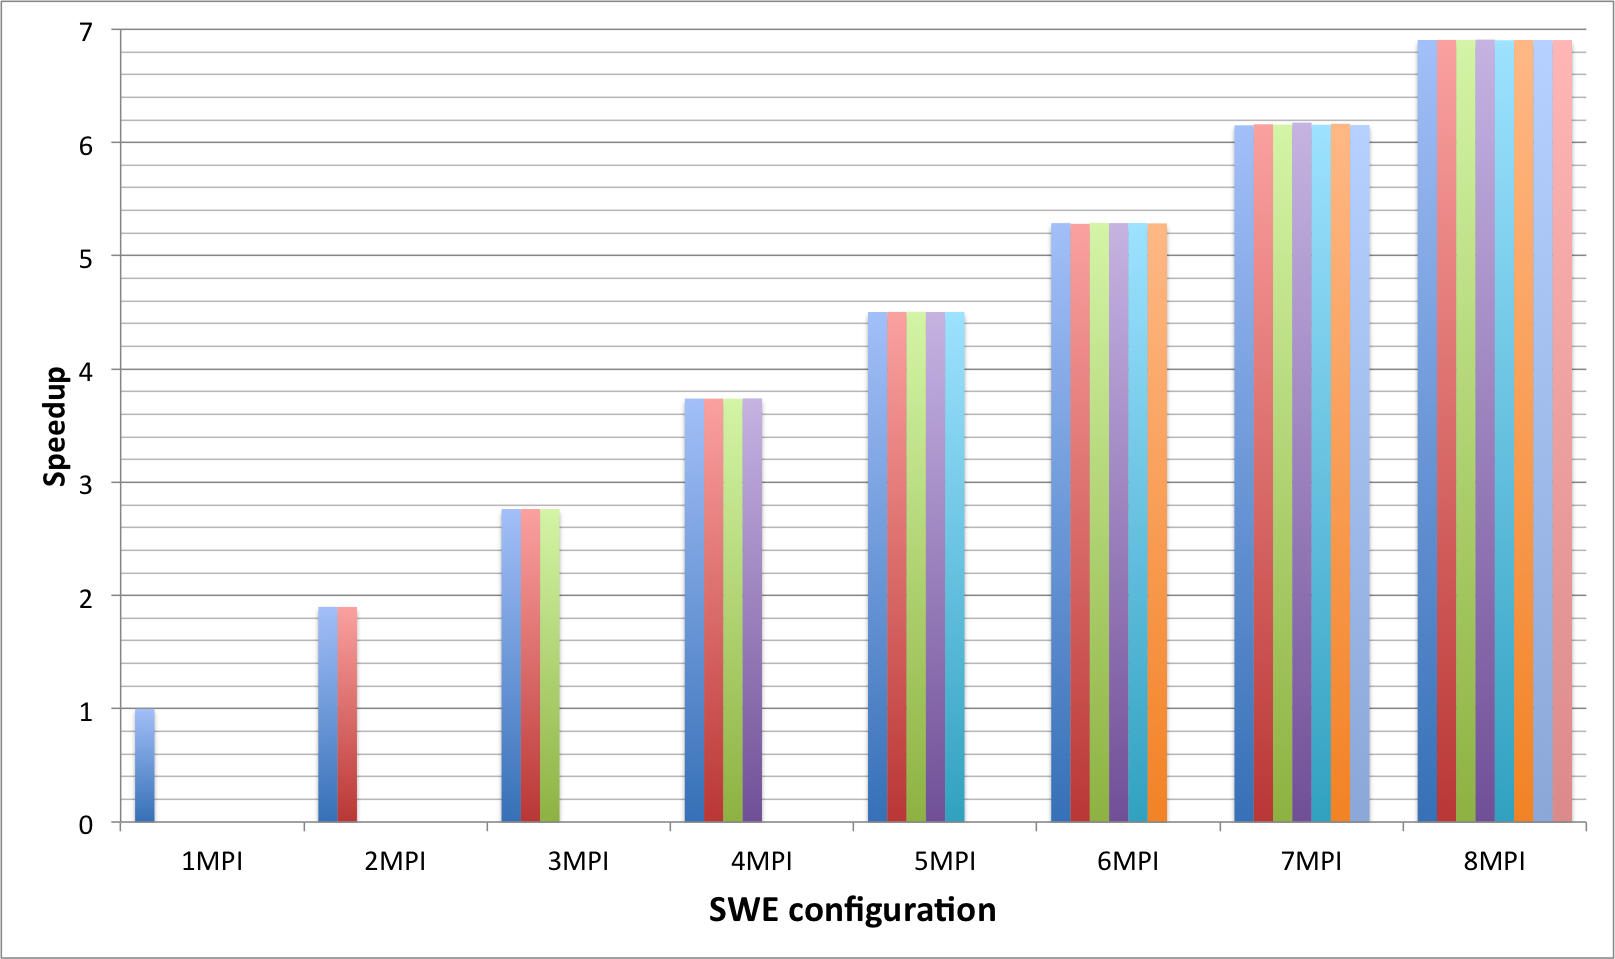
\includegraphics[height=6cm]{figures/mpi_sumatra} 
}}
\quad
\mbox{
\subfigure[Tohoku tsunami simulation]{
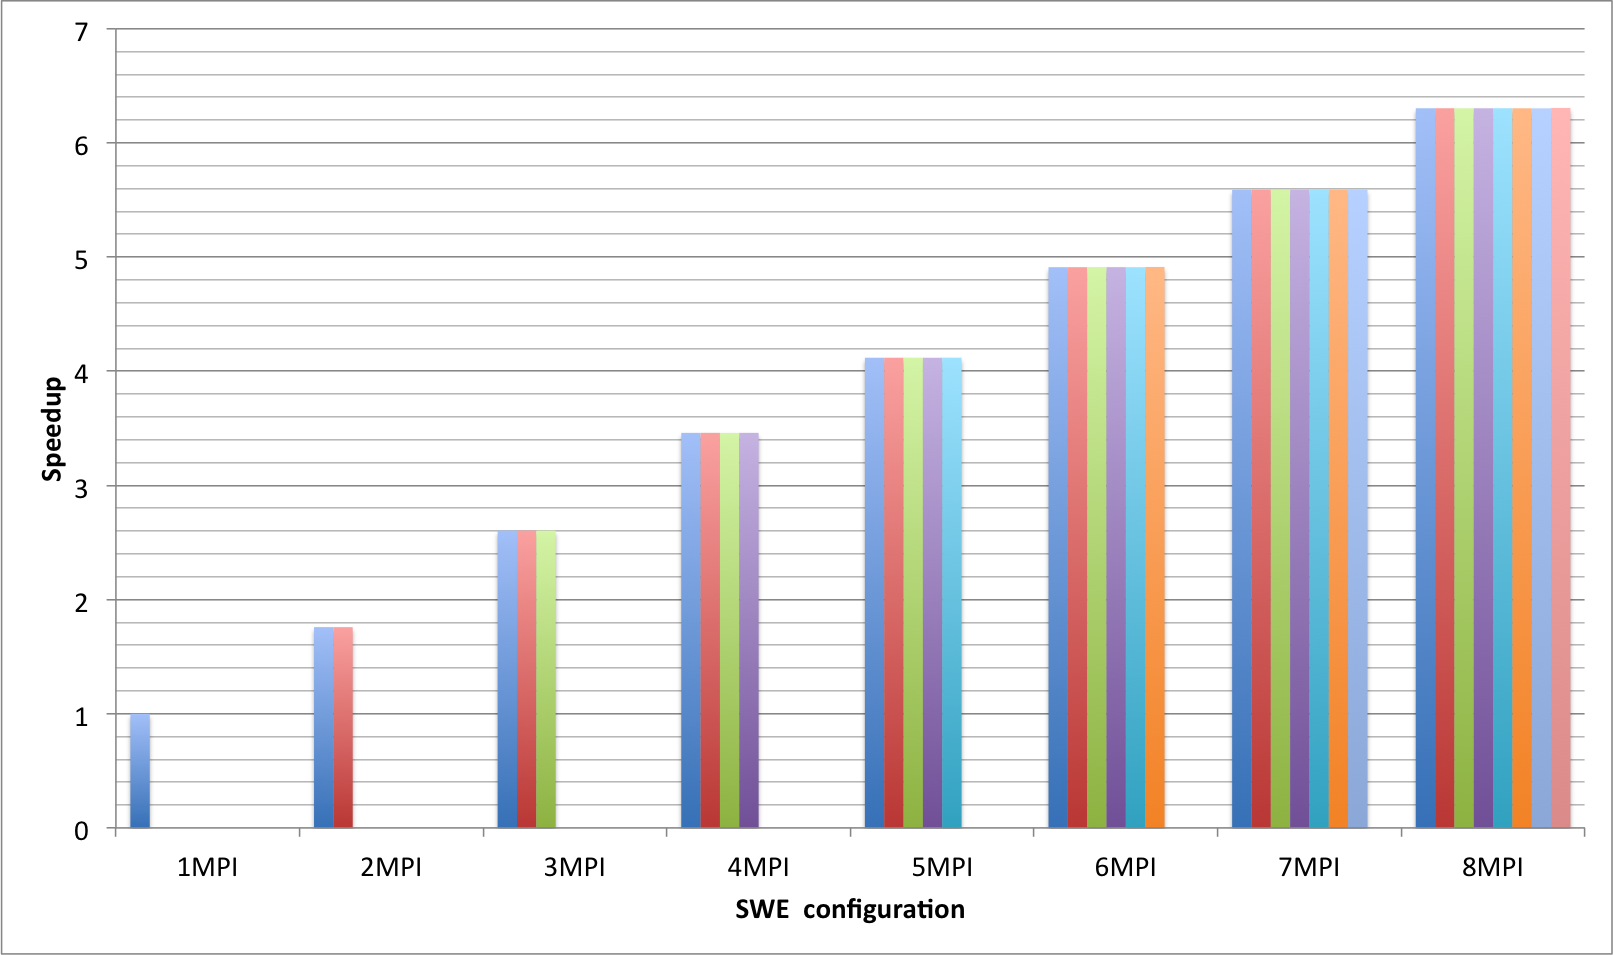
\includegraphics[height=6cm]{figures/mpi_tohoku} 
}}
\caption{Observed speedups with different number of CPU processes on \emph{Tesla-CMC}}
\label{fig:mpi_speedup}
\end{figure}

\begin{figure}
\centering
\mbox{
\subfigure[Sumatra tsunami simulation]{
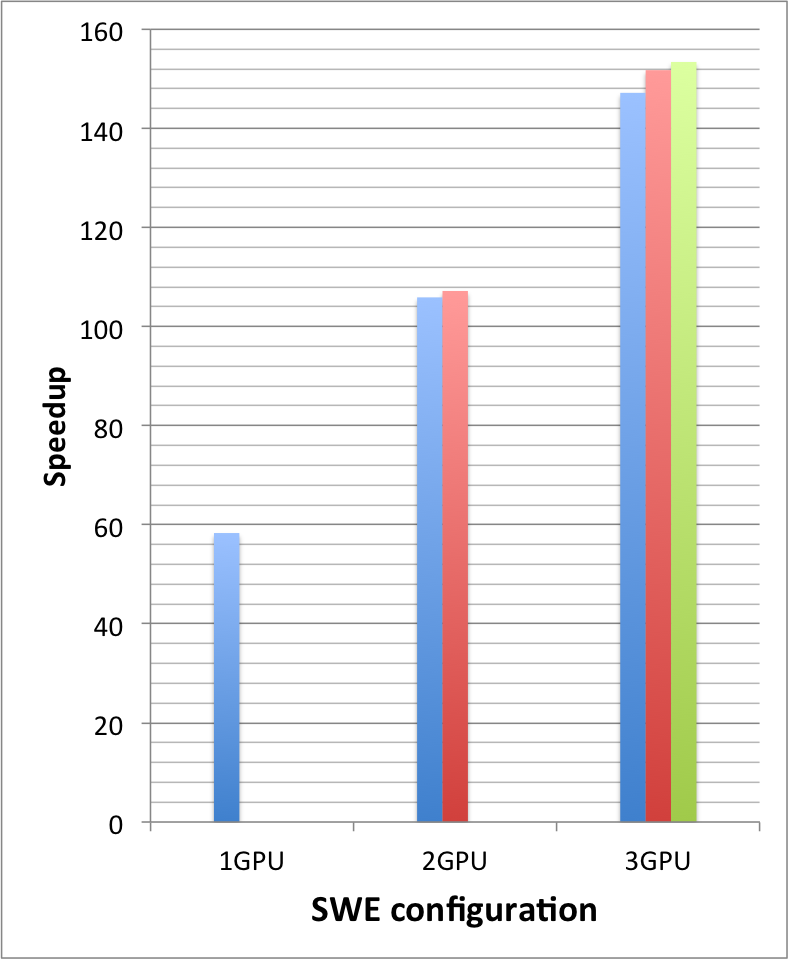
\includegraphics[height=6cm]{figures/gpu_sumatra} 
}}
\quad
\mbox{
\subfigure[Tohoku tsunami simulation]{
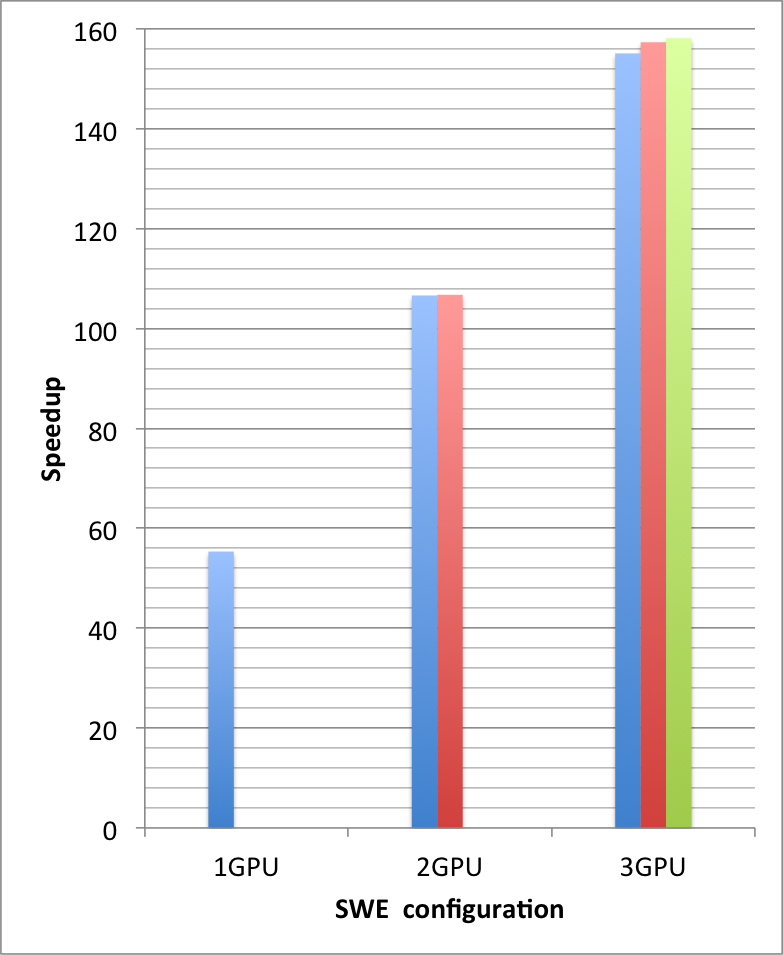
\includegraphics[height=6cm]{figures/gpu_tohoku} 
}}
\caption{Observed speedups with different number of GPUs on \emph{Tesla-CMC}}
\end{figure}

\begin{figure}
\centering
\mbox{
\subfigure[Parallelization using multiple CPU processes]{
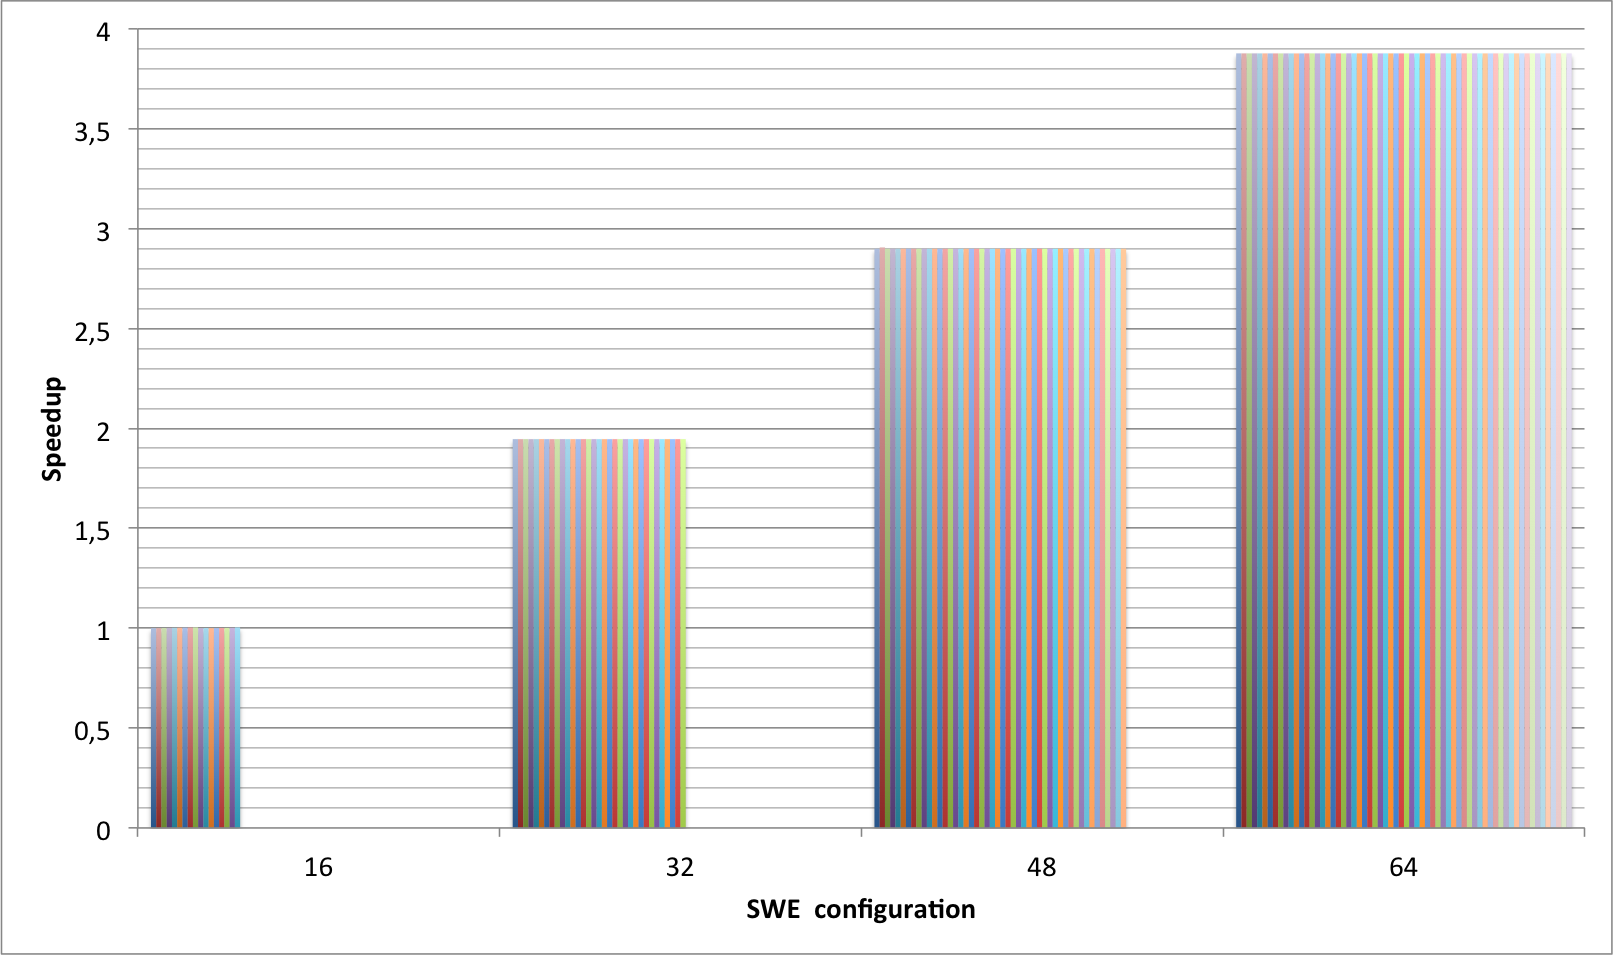
\includegraphics[height=6cm]{figures/todi_mpi}
}}
\quad
\mbox{
\subfigure[Parallelization using multiple CPU processes with GPUs]{
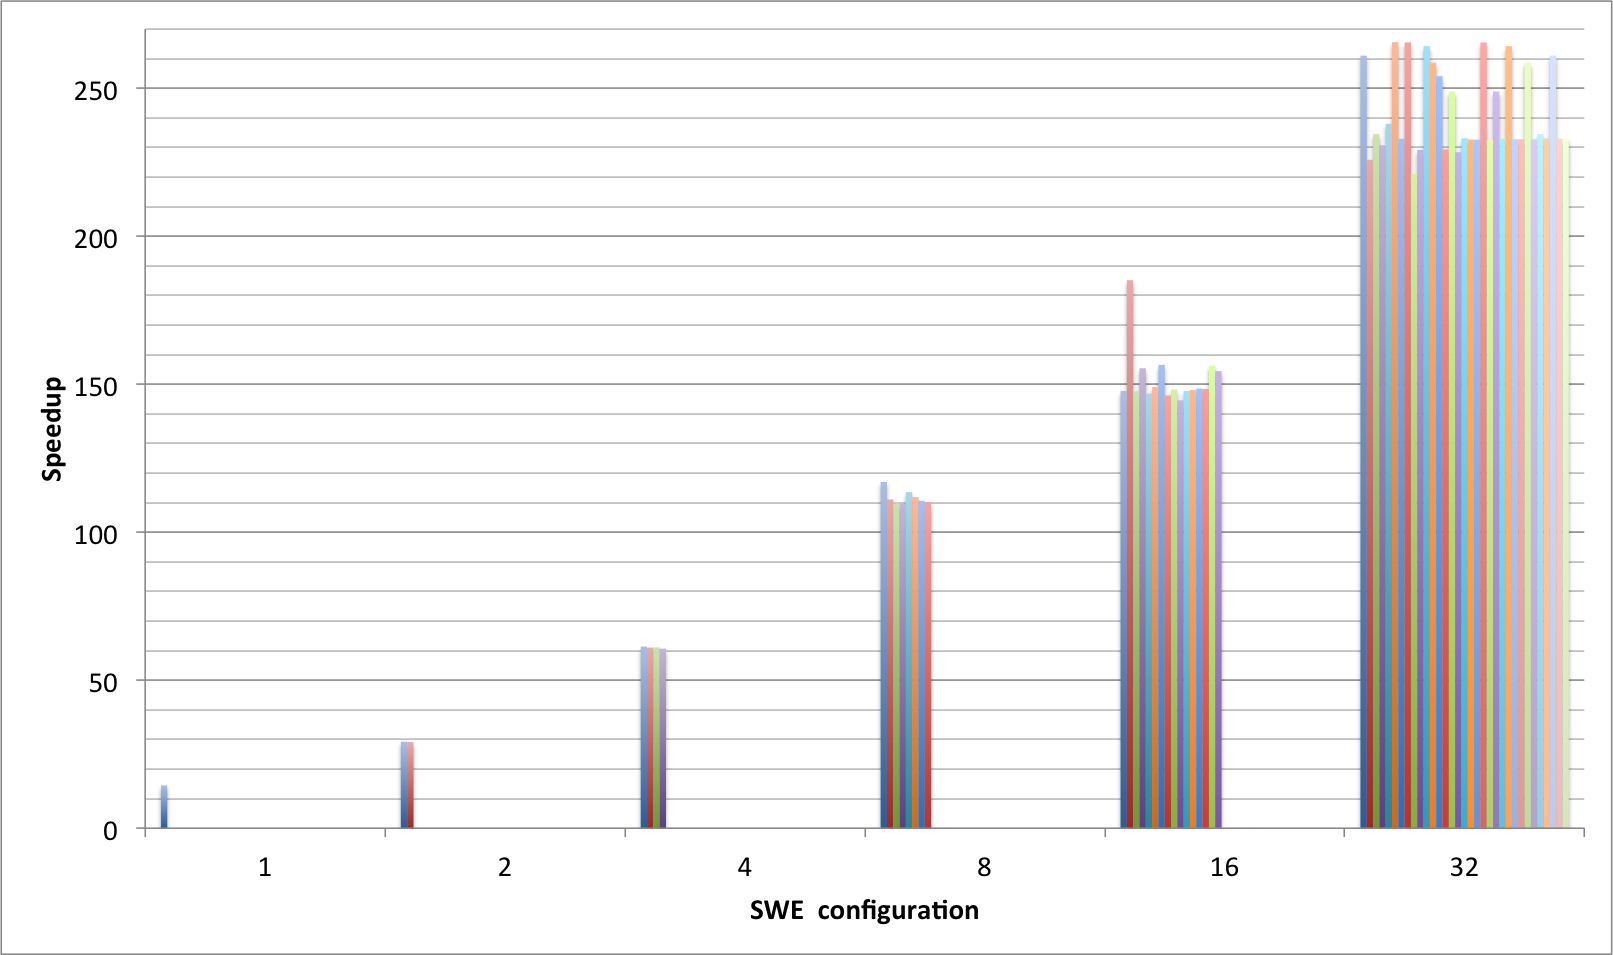
\includegraphics[height=6cm]{figures/todi_gpu} 
}}
\caption{Observed speedups with different configurations on \emph{Todi Cray XK-7}}
\end{figure}

\end{document}

